\documentclass{article}

% Language setting
% Replace `english' with e.g. `spanish' to change the document language
\usepackage[english]{babel}

% Set page size and margins
% Replace `letterpaper' with `a4paper' for UK/EU standard size
\usepackage[letterpaper,top=2cm,bottom=2cm,left=3cm,right=3cm,marginparwidth=1.75cm]{geometry}
\usepackage{CJKutf8}
% Useful packages
\usepackage{amsmath}
\usepackage{graphicx}
\usepackage{setspace}
\usepackage[colorlinks=true, allcolors=blue]{hyperref}
\usepackage[export]{adjustbox}


\title{\Huge Synoptic Meteorology HW5}
\author{B10209040 陳彥倫}

\begin{document}
\begin{CJK*}{UTF8}{bsmi}
\maketitle


\section{Skew-T before adiabatic lifting}
\begin{spacing}{1.5}
下圖左一及左二顯示了此時此地在被地形舉升前的探空圖。可以發現環境氣溫從地表到高空始終大於絕熱上升之氣塊溫度。
且另外繪製$\theta_e$跟$z$的關係圖,在我們關注的1000hPa至500hPa的空氣層之$\frac{\delta\theta_e}{\delta z}
<0$代表此空氣層的性質為潛在不穩定。
\end{spacing}


\section{Skew-T after adiabatic lifting}
\begin{spacing}{1.5}
右圖則為1000hpa至500hpa空氣層整層抬升1000m後之結果。將500hPa以下之資料點以壓高公式計算出那一空氣層抬升後的高度
,溫度及露點溫度的部分則分別沿乾絕熱遞減率(9.8 degC/km)及等混合比線(2 degC/km)下降,若於舉升1000m前溫度即等於
露點則繼續以濕絕熱遞減率下降。
\end{spacing}


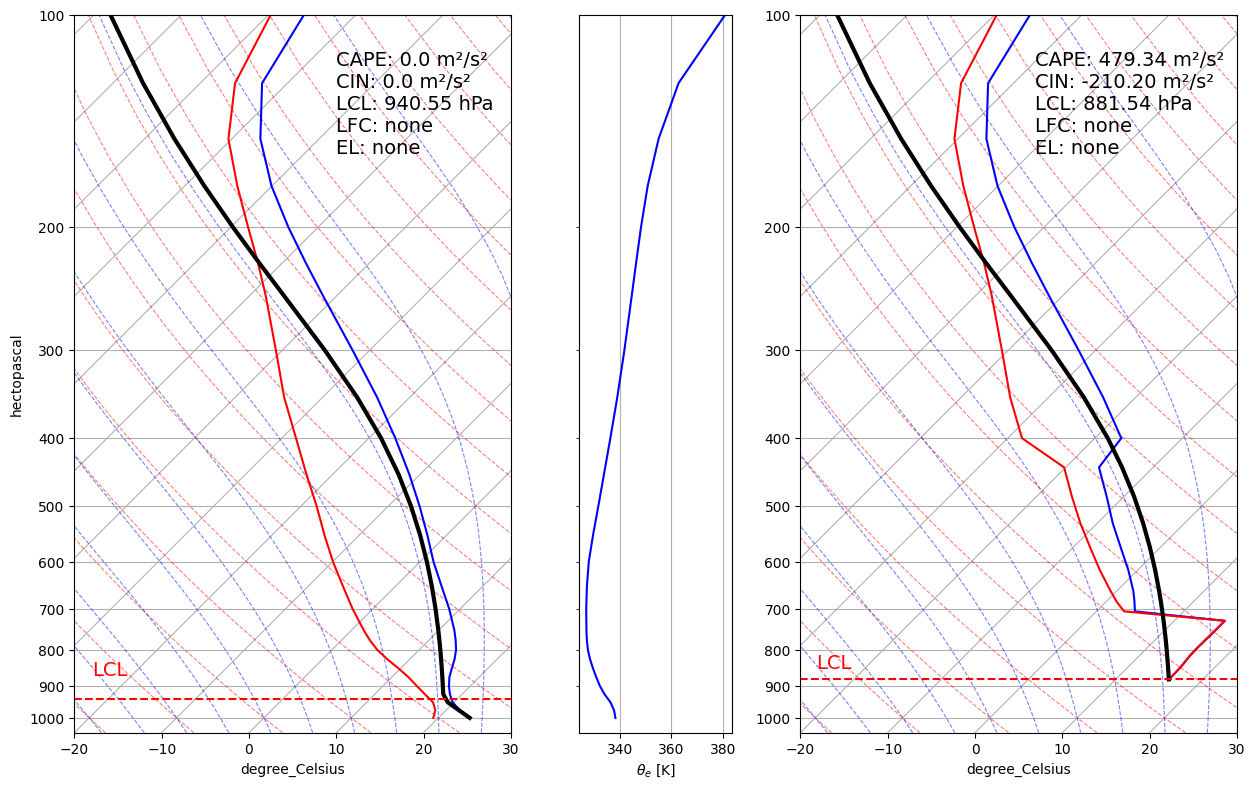
\includegraphics[width=1\linewidth, center]{output.png}


\end{CJK*}
\end{document}